% =====================================================================
%  PEDOMAN PENULISAN SKRIPSI
%  Program Studi Rekayasa Sistem Komputer, Fakultas Teknik, UM Buton
%  Kompilasi PDF : xelatex (lihat menu.sh)   |   Word : pandoc (lihat menu.sh)
% =====================================================================
\documentclass[12pt,a4paper]{report}
\usepackage{skripsi}
\usepackage[a4paper,left=4cm,right=3cm,top=4cm,bottom=3cm]{geometry}
\usepackage{tocloft}

% ---------- Data dosen & peran (common/dosen.tex, common/peran.tex) ----------
% =====================================================================
%  DAFTAR DOSEN  --  Program Studi Rekayasa Sistem Komputer, UM Buton
%  Satu dosen = dua makro:  \dsnKunci (nama dan gelar)  dan  \nidnKunci (NIDN).
%  Tambah dosen baru dengan menyalin dua baris di bawah. Peran (pembimbing, penguji, dst.)
%  diatur di peran.tex atau lewat  ./menu.sh  ->  "Atur dosen / peran".
% =====================================================================
\newcommand{\dsnAwaluddin}{Muhammad Awaluddin, S.Kom., M.Kom}
\newcommand{\nidnAwaluddin}{0909038201}
\newcommand{\dsnDarmawan}{Darmawan, S.Kom., M.Kom}
\newcommand{\nidnDarmawan}{0911048204}
\newcommand{\dsnRando}{Rando, S.Kom., M.Eng.}
\newcommand{\nidnRando}{0911069501}
\newcommand{\dsnSaidi}{La Ode Muhammad Saidi, S.Si., M.Kom}
\newcommand{\nidnSaidi}{0913038905}
\newcommand{\dsnDidin}{Didin Adri, S.Si., M.Sc}
\newcommand{\nidnDidin}{0930088802}
\newcommand{\dsnHibrian}{Muhammad Hibrian Wiwi, S.T., M.Kom}
\newcommand{\nidnHibrian}{0930129003}
\newcommand{\dsnRasyid}{Muhammad Abdur Rasyid Asruddin, S.T., M.Kom}
\newcommand{\nidnRasyid}{6641774675130242}
% Dekan Fakultas Teknik
\newcommand{\dsnAgusman}{Agusman, S.T., M.M}
\newcommand{\nidnAgusman}{0917088206}

% =====================================================================
%  PERAN DOSEN  --  dipakai otomatis di sampul, lembar persetujuan/pengesahan,
%  kata pengantar, dan abstrak semua dokumen.
%  Isi dengan kunci dosen dari dosen.tex, mis.  \dsnAwaluddin  dan  \nidnAwaluddin.
%  Atau jalankan  ./menu.sh  lalu pilih "Atur dosen / peran"  (berkas ini ditulis ulang otomatis).
% =====================================================================
\newcommand{\PembimbingI}{…………………}\newcommand{\PembimbingInidn}{……………………}
\newcommand{\PembimbingII}{…………………}\newcommand{\PembimbingIInidn}{……………………}
\newcommand{\PengujiI}{…………………}\newcommand{\PengujiInidn}{……………………}
\newcommand{\PengujiII}{…………………}\newcommand{\PengujiIInidn}{……………………}
\newcommand{\KetuaProdi}{…………………}\newcommand{\KetuaProdinidn}{……………………}
\newcommand{\Dekan}{\dsnAgusman}\newcommand{\Dekannidn}{\nidnAgusman}


% ---------- Makro yang ikut dibaca pandoc (jangan dipindah ke .sty) ----------
\newcommand{\logo}[1]{
\includegraphics[width=#1]{../gambar/logo-umbuton.png}}
\newcommand{\babtp}[1]{\chapter*{#1}\addcontentsline{toc}{chapter}{#1}}
\newcommand{\lampiran}[2]{\babtp{LAMPIRAN #1. #2}\setcounter{figure}{0}\setcounter{table}{0}\renewcommand{\thefigure}{L#1.\arabic{figure}}\renewcommand{\thetable}{L#1.\arabic{table}}}   % nomor gambar/tabel di lampiran: L2.1

% ---------- Tata letak khusus LaTeX ----------
\setstretch{1.9}                       % setara "2 spasi" di Microsoft Word
\setlength{\parindent}{1.27cm}         % alinea: tab stop 0,5"
\setlength{\parskip}{0pt}
\hyphenpenalty=10000 \exhyphenpenalty=10000 \emergencystretch=4em   % tanpa pemenggalan kata
\setlist{nosep,leftmargin=1.27cm,itemsep=0pt,topsep=0pt}
\setcounter{secnumdepth}{3}
\counterwithin{figure}{chapter}   % nomor gambar/tabel = nomor bab . urutan di bab itu (Gambar 1.1, Tabel 2.3)
\counterwithin{table}{chapter}
\renewcommand{\thefigure}{\arabic{chapter}.\arabic{figure}}
\renewcommand{\thetable}{\arabic{chapter}.\arabic{table}}
\setcounter{tocdepth}{2}
\renewcommand{\thechapter}{\Roman{chapter}}
\renewcommand{\thesection}{\arabic{chapter}.\arabic{section}}

\titleformat{\chapter}[display]{\centering\bfseries\singlespacing}{BAB \thechapter}{12pt}{}
\titleformat{name=\chapter,numberless}[block]{\centering\bfseries\singlespacing}{}{0pt}{}
\titlespacing{\chapter}{0pt}{0pt}{24pt}
\titleformat{\section}{\bfseries\singlespacing}{\thesection}{1em}{}
\titleformat{\subsection}{\bfseries\singlespacing}{\thesubsection}{1em}{}
\titleformat{\subsubsection}{\itshape\singlespacing}{\thesubsubsection}{1em}{}
\titlespacing{\section}{0pt}{18pt}{12pt}
\titlespacing{\subsection}{0pt}{18pt}{12pt}
\titlespacing{\subsubsection}{0pt}{12pt}{6pt}

\renewcommand{\arraystretch}{1.2}
\captionsetup{font=singlespacing,labelsep=period,skip=6pt}
\captionsetup[table]{justification=raggedright,singlelinecheck=false,position=above}
\captionsetup[figure]{justification=centering}

% nomor halaman: awal bab = tengah bawah (gaya "plain"); halaman setelahnya = kanan atas (gaya "isi")
\setlength{\headheight}{14.5pt}
\fancypagestyle{plain}{\fancyhf{}\fancyfoot[C]{\thepage}\renewcommand{\headrulewidth}{0pt}}
\fancypagestyle{isi}{\fancyhf{}\fancyhead[R]{\thepage}\renewcommand{\headrulewidth}{0pt}}
\pagestyle{plain}

% daftar isi
\renewcommand{\cftchapfont}{\bfseries}
\renewcommand{\cftchappagefont}{\bfseries}
\renewcommand{\cftchappresnum}{BAB~}
\setlength{\cftchapnumwidth}{4.6em}
\renewcommand{\cftchapleader}{\cftdotfill{\cftdotsep}}
\setlength{\cftbeforechapskip}{8pt}
\setlength{\cftbeforesecskip}{3pt}
\setlength{\cftbeforesubsecskip}{2pt}
\setlength{\cftsecindent}{0pt}
\setlength{\cftsecnumwidth}{3em}
\setlength{\cftsubsecindent}{3em}
\setlength{\cftsubsecnumwidth}{3.6em}

\begin{document}

% ============================ SAMPUL ============================
\thispagestyle{empty}
\begin{ruang}{1.0}\end{ruang}
\begin{tengah}
\textbf{\large PEDOMAN PENULISAN SKRIPSI}
\end{tengah}
\begin{ruang}{2.5}\end{ruang}
\begin{tengah}
\logo{4.5cm}
\end{tengah}
\begin{ruang}{3.5}\end{ruang}
\begin{tengah}
\textbf{PROGRAM STUDI REKAYASA SISTEM KOMPUTER}

\textbf{FAKULTAS TEKNIK}

\textbf{UNIVERSITAS MUHAMMADIYAH BUTON}

\textbf{BAUBAU}

\textbf{2021}
\end{tengah}
\begin{akhirsampul}\end{akhirsampul}

% ============================ HALAMAN PENGAJUAN ============================
\babtp{HALAMAN PENGAJUAN}
\begin{ruang}{0.4}\end{ruang}
\begin{tengah}
\textbf{SEMINAR PROPOSAL/HASIL/AKHIR}

\textbf{JUDUL PENELITIAN}
\end{tengah}
\begin{ruang}{0.8}\end{ruang}
\begin{tengah}
\logo{4cm}
\end{tengah}
\begin{ruang}{1.2}\end{ruang}
\begin{tengah}
\textit{Disusun oleh:}

\textbf{NAMA MAHASISWA}

\textbf{NPM}
\end{tengah}
\begin{ruang}{1.8}\end{ruang}
\begin{tengah}
\textbf{PROGRAM STUDI REKAYASA SISTEM KOMPUTER}

\textbf{FAKULTAS TEKNIK}

\textbf{UNIVERSITAS MUHAMMADIYAH BUTON}

\textbf{BAUBAU}

\textbf{2021}
\end{tengah}

% ============================ HALAMAN PENGESAHAN ============================
\babtp{HALAMAN PENGESAHAN}
\begin{ruang}{0.4}\end{ruang}
\begin{tengah}
\textbf{SEMINAR PROPOSAL/HASIL/AKHIR}

\textbf{JUDUL PENELITIAN}

Disusun dan diajukan oleh:

\textbf{NAMA MAHASISWA}

\textbf{NPM}
\end{tengah}
\begin{ruang}{0.4}\end{ruang}
\begin{tengah}
\logo{3cm}
\end{tengah}
\begin{ruang}{0.5}\end{ruang}
\begin{tengah}
Menyetujui

Komisi Penasihat
\end{tengah}

\begin{tanpagaris}\begin{tabelpusat}
\begin{longtable}{@{}>{\centering\arraybackslash}p{0.48\linewidth}>{\centering\arraybackslash}p{0.48\linewidth}@{}}
\textbf{Pembimbing I}\newline ~\newline ~\newline \PembimbingI\newline NIDN. \PembimbingInidn &
\textbf{Pembimbing II}\newline ~\newline ~\newline \PembimbingII\newline NIDN. \PembimbingIInidn \\
~ & ~ \\
\textbf{Ketua Program Studi}\newline ~\newline ~\newline \KetuaProdi\newline NIDN. \KetuaProdinidn &
\textbf{Dekan Fakultas Teknik}\newline ~\newline ~\newline \Dekan\newline NIDN. \Dekannidn \\
\end{longtable}
\end{tabelpusat}\end{tanpagaris}

% ============================ KATA PENGANTAR ============================
\babtp{KATA PENGANTAR}

Buku Pedoman Penulisan Skripsi Fakultas Teknik Universitas Muhammadiyah Buton diterbitkan untuk menyempurnakan cara penulisan skripsi oleh mahasiswa dan sebagai pedoman bagi dosen dalam melaksanakan tugas pembimbingan.

Diterbitkannya Buku Pedoman Penulisan Skripsi berdasarkan SK Dekan tentang ……………………………………………………………….

Akhirnya kami berharap agar Buku Pedoman ini dapat berfungsi sebagai acuan dalam pelaksanaan pendidikan baik untuk Pimpinan Fakultas, Program Studi, Dosen dan Mahasiswa.

\begin{kanan}
Fakultas Teknik\\
Universitas Muhammadiyah Buton\\
Dekan,

\textbf{\Dekan}\\
NIDN : \Dekannidn
\end{kanan}

% ============================ DAFTAR ISI ============================
\begin{daftarisi}\end{daftarisi}

\begin{akhirdepan}\end{akhirdepan}
\pagestyle{isi}

% ============================ BAB I ============================
\chapter{PENDAHULUAN}

\section{Pengertian}
Skripsi adalah karya tulis ilmiah yang disusun berdasarkan hasil penelitian lapang atau laboratorium yang dilengkapi dengan analisis statistik inferensial untuk pendekatan kuantitatif dan deskriptif untuk pendekatan kualitatif.

\section{Tujuan}
Tujuan pembuatan skripsi adalah:
\begin{enumerate}
\item Agar mahasiswa memiliki kemampuan, keterampilan dan pengalaman untuk memecahkan salah satu masalah dalam bidang teknik sipil.
\item Memberi kesempatan kepada mahasiswa untuk dapat memahami salah satu cabang ilmu teknik sipil.
\item Agar mahasiswa memiliki kemampuan untuk menyusun suatu karya ilmiah berdasarkan metode keilmuan.
\end{enumerate}

\section{Sistematika Penulisan Skripsi}
Sebelum membuat suatu usulan penelitian, perlu diingat bahwa antara judul penelitian, latar belakang, masalah, tujuan dan kegunaan, kerangka pikir, hipotesis, serta materi dan metode penelitian yang direncanakan harus runtut yang bertujuan untuk memudahkan evaluasi tentang dapat atau tidaknya penelitian dilakukan. Usulan penelitian harus sudah disetujui oleh dosen pembimbing sebelum penelitian dilaksanakan.

\subsection{Halaman Sampul}
Contoh halaman sampul usulan penelitian sesuai dengan halaman sampul Pedoman Penulisan Skripsi Universitas Muhammadiyah Buton.

\subsection{Halaman Pengajuan}
Halaman Pengajuan memuat judul penelitian, kata-kata Usulan Penelitian, Oleh, nama mahasiswa, dan NPM, sesuai dengan Halaman Pengajuan Pedoman Penulisan Skripsi Universitas Muhammadiyah Buton.

\subsection{Halaman Pengesahan}
Halaman ini memuat judul penelitian, kata-kata Usulan Penelitian, Oleh, nama mahasiswa, NPM, kolom tanda tangan persetujuan para dosen pembimbing, Ketua Program Studi dan Dekan, sesuai dengan Halaman Pengesahan Pedoman Penulisan Skripsi Universitas Muhammadiyah Buton.

\subsection{Pendahuluan}
Pendahuluan disusun secara sistematis dan terarah dalam urutan logika yang memberi justifikasi terhadap kerangka pikir, latar belakang masalah, tujuan, kegunaan, rumusan masalah dan hipotesis penelitian yang diajukan.

Pendahuluan harus menguraikan secara jelas dan ringkas tentang latar belakang masalah yang dihadapi dan perlunya penelitian dilakukan untuk memecahkan masalah yang dihadapi. Uraian tersebut dapat dibuat berdasarkan kepustakaan, kenyataan di lapang atau kombinasi keduanya.

Tujuan dan manfaat penelitian harus pula dipaparkan secara jelas tetapi singkat. Bab Pendahuluan ini juga dapat memuat hipotesis.

\subsection{Latar Belakang}
Latar belakang berisi justifikasi terhadap penelitian yang akan dilakukan dalam kaitannya dengan tujuan penelitian yang diajukan, uraian yang mengemukakan permasalahan-permasalahan yang secara umum dihadapi dan terkait dengan judul penelitian. Pendapat peneliti baik yang ditulis dalam bentuk \textit{textbook} maupun jurnal hasil penelitian yang relevan dengan judul penelitian yang diusulkan perlu juga dikemukakan.

\subsection{Rumusan Masalah}
Rumusan masalah didasarkan pada latar belakang yang telah dikemukakan. Dari latar belakang masalah disusun satu atau lebih rumusan masalah. Bentuk rumusan masalah umumnya berupa pertanyaan, dapat pula berbentuk pernyataan yang memerlukan jawaban melalui penelitian ilmiah.

\subsection{Tujuan Penelitian}
Tujuan penelitian disusun berdasarkan rumusan masalah, sehingga perlu adanya konsistensi antara rumusan masalah dengan tujuan penelitian. Tujuan penelitian menyatakan segala sesuatu yang ingin diperoleh dan diketahui melalui penelitian. Tujuan penelitian berupa kalimat pernyataan singkat, jelas dan spesifik tentang apa yang ingin diketahui dari kegiatan penelitian.

\subsection{Manfaat Penelitian}
Manfaat penelitian menguraikan tentang manfaat yang diperoleh apabila tujuan penelitian tercapai dan difokuskan pada pengembangan keilmuan, informasi bagi pembuat kebijakan dan umpan balik bagi para pengguna terutama dalam pembangunan teknik sipil.

\subsection{Kerangka Pikir}
Kerangka pikir menguraikan tentang hasil-hasil penelitian atau pendapat terdahulu yang serupa, yang dapat digunakan untuk landasan berpijak dalam menentukan pengajuan hipotesis. Kerangka pemikiran merupakan justifikasi ilmiah terhadap penelitian yang akan dilakukan. Pada hakekatnya kerangka pikir harus didukung oleh landasan teoritis dan ditunjang oleh landasan informasi yang bersumber dari berbagai laporan ilmiah, sehingga menghasilkan suatu pemikiran baru dalam pendekatannya. Pemikiran baru tersebut dapat merupakan modifikasi atau penyempurnaan, gabungan atau perombakan total terhadap pendekatan lama yang tercermin dalam hipotesis penelitian.

% ============================ BAB II ============================
\chapter{ISI PENULISAN SKRIPSI}

Penulisan skripsi merupakan bagian terpenting dari seluruh proses kegiatan penelitian yang telah dilakukan, karena dalam laporan itu semua ide dan hasil kegiatan dapat disampaikan kepada orang lain, termasuk orang yang disiplin ilmunya berbeda. Laporan harus jelas mengungkapkan semua kegiatan dan hasil-hasilnya secara sistematis, efisien dan efektif menggunakan Bahasa Indonesia yang baik dan benar.

\section{Bagian Isi}

\subsection{Tinjauan Pustaka}
Tinjauan pustaka hanya berisikan teori-teori yang mendukung penelitian. Penulis wajib menyederhanakan uraian dari pustaka yang diambil asalkan tanpa mengubah maksudnya. Tinjauan pustaka dapat memuat hal-hal yang sejalan maupun bertentangan dengan pendapat peneliti lain atau membenarkan pendekatan yang dipakai untuk memecahkan masalah yang dihadapi, dengan tujuan mempertahankan alur uraian supaya sistematis dengan tidak mengubah pengertian suatu masalah sesuai pustaka yang dipakai. Pustaka yang digunakan harus orisinal (tidak mengutip dari skripsi) dan mutakhir.

Informasi dalam tinjauan pustaka dapat terdiri atas kutipan dari bab tertentu dari buku, majalah ilmiah, laporan penelitian atau jurnal, dapat pula laporan yang tidak diterbitkan, komunikasi pribadi, dan internet. Kutipan informasi di atas disusun secara runtut sehingga memberikan alur pikiran yang jelas.

Tinjauan pustaka disajikan secara sistematis dan jelas tentang hal-hal yang mendukung penelitian. Peneliti dituntut agar menggunakan sumber informasi atau pustaka asli dan mutakhir.

Kutipan informasi yang disajikan dalam tinjauan pustaka harus jelas sumbernya. Nama sumber disajikan di depan atau di belakang kalimat, beserta tahun penerbitannya. Tata cara penulisan pustaka adalah sebagai berikut:
\begin{enumerate}
\item Nama penulis satu atau dua orang ditulis semua.
\item Nama penulis lebih dari dua orang: nama semua penulis dicantumkan pada saat kutipan itu ditulis pertama kali, untuk selanjutnya hanya penulis pertama yang ditulis kemudian diikuti \textit{dkk.} (pustaka berbahasa Indonesia) atau \textit{et al.} (untuk pustaka berbahasa asing).
\item Nama penulis lebih dari satu ditulis “dan” (pustaka berbahasa Indonesia) atau “\textit{and}” (untuk pustaka berbahasa asing).
\item Penulisan tahun pustaka dimulai dari yang termuda.
\end{enumerate}
Contoh:
\begin{enumerate}
\item Sanford \textit{and} Woodgate (1993) menyatakan bahwa masa kebuntingan induk kelinci tergantung pada kualitas makanan, terutama pada dua minggu terakhir masa kebuntingan.
\item Melalui pemecahan kulit telur, kualitas telur dapat dilihat secara langsung (Buckle, Edward, Fleet \textit{and} Wooton, 1976; Oluyemi \textit{and} Robert, 1981).
\end{enumerate}
Tinjauan pustaka disusun menjadi beberapa subbab, sehingga menghasilkan wawasan yang dapat dipakai dalam pembahasan hasil penelitian.

\subsection{Penelitian Terdahulu}
Penelitian terdahulu berisi penelitian-penelitian sejenis yang pernah dilakukan. Dalam penelitian terdahulu penulis wajib memasukkan minimal empat penelitian dalam kurun waktu tidak lebih dari 10 tahun terakhir. Penelitian yang ditulis cukup nama peneliti, judul penelitian dan kesimpulan hasil penelitian, dibagi dalam satu paragraf untuk satu penelitian. Sumber yang digunakan boleh berasal dari skripsi, tesis, disertasi maupun jurnal ilmiah.

\subsection{Metode Penelitian}
Pada bab ini dicantumkan lokasi dan waktu penelitian, materi penelitian, metode penelitian, variabel pengamatan, analisis data dan batasan istilah. Hal-hal tersebut diuraikan secara jelas sehingga orang lain dapat mengulangi penelitian yang telah dikerjakan dengan cara yang sama bila ingin melakukan pengkajian ulang. Cara penulisan materi, bahan dan alat disusun ke samping, sedangkan cara penulisan prosedur analisis atau jalannya penelitian disusun ke bawah sesuai urutan kerja.

\subsubsection{Lokasi dan Waktu Penelitian}
Lokasi penelitian hendaknya disebutkan dengan jelas dan lengkap. Khusus penelitian lapang hendaknya disebutkan secara administratif, geografis dan keterangan topografis, klimatologis berikut sumber informasinya. Waktu yang dimaksudkan di sini adalah lama/masa pengumpulan data.

\subsubsection{Materi Penelitian}
Materi penelitian menjelaskan tentang sampel yang diteliti, bahan dan peralatan. Sampel penelitian harus diterangkan mengenai komoditas yang diteliti, jumlah, cara perolehan dan keterangan lain yang mendukung. Bahan penelitian dideskripsikan secara jelas nama ilmiah (\textit{scientific name}) dan nama produsen. Peralatan penelitian disebutkan nama dan spesifikasinya serta nama produsen.

\subsubsection{Metode Penelitian}
Metode penelitian dilakukan dengan pendekatan kuantitatif maupun kualitatif sesuai dengan masalah yang dirumuskan dan tujuan penelitian. Metode penelitian meliputi: teknik pengambilan sampel, metode penelitian (sesuai dengan tujuan penelitian), perlakuan sampel, macam perlakuan dan ulangan, rancangan percobaan, prosedur pengumpulan data dan analisis.

Sampel penelitian didasarkan pada kepentingan bidang studi, unit percobaan dan analisis data yang dipakai disesuaikan dengan tujuan yang dicapai dalam penelitian. Batasan-batasan istilah merupakan definisi/pengertian yang digunakan sesuai dengan penelitian.

\subsection{Hasil Penelitian dan Pembahasan}
Hasil penelitian berisi data primer dan atau sekunder. Hasil penelitian yang bersifat kualitatif diungkapkan dalam bentuk narasi ilmiah sesuai dengan tujuan penelitian, sedangkan yang bersifat kuantitatif diungkapkan dalam bentuk tabel, grafik dan foto-foto. Data yang dikemukakan dalam bab hasil dan pembahasan hendaknya bukan data murni, melainkan hasil olahan statistik, sedangkan data laboratorium/lapangan yang diperoleh dapat dimasukkan dalam bentuk data murni.

Penyajian hasil penelitian atau pengamatan dapat berupa teks, tabel, gambar, grafik dan foto. Hasil penelitian dapat memuat data utama, data penunjang, dan pelengkap yang diperlukan untuk memperkuat hasil penelitian menggunakan uji statistik, apabila dalam kondisi tertentu dimungkinkan tidak menggunakan uji statistik. Narasi hasil penelitian memuat ulasan makna yang terdapat dalam tabel, gambar, grafik dan foto.

Pembahasan dikemukakan secara komprehensif terkait dengan hasil penelitian diperkuat dengan hasil-hasil peneliti lain atau \textit{textbook}. Ulasan dalam pembahasan dapat berupa penjelasan teoritis baik secara kualitatif dan kuantitatif.

\subsection{Variabel Pengamatan}
Variabel diartikan sebagai segala sesuatu yang menjadi obyek pengamatan penelitian. Hal-hal yang merupakan variabel dalam suatu penelitian ditentukan oleh landasan teoritis yang diambil dan secara eksplisit telah dinyatakan dalam rumusan hipotesis. Klasifikasi variabel menurut perannya perlu dikemukakan dengan jelas, sehingga masing-masing variabel bebas dan variabel tidak bebas dengan mudah dapat diidentifikasi.

\subsection{Penulisan Flowchart}
\textit{Processing symbols} menunjukkan jenis operasi pengolahan dalam suatu prosedur. Berikut beberapa simbol yang umum digunakan dalam penulisan sebuah skripsi.

\begin{tanpagaris}
\begin{longtable}{@{}p{0.24\linewidth}p{0.72\linewidth}@{}}

\includegraphics[width=2.4cm]{../gambar/simbol-1.png} & \textbf{\textit{Symbol Process}} (simbol yang menunjukkan pengolahan yang dilakukan oleh komputer) \\
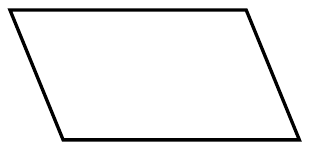
\includegraphics[width=2.4cm]{../gambar/simbol-2.png} & \textbf{\textit{Symbol Input/Output}} (simbol yang menunjukkan proses input atau output) \\
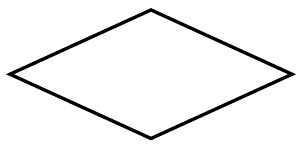
\includegraphics[width=2.4cm]{../gambar/simbol-3.png} & \textbf{\textit{Symbol Decision}} (simbol untuk kondisi yang akan menghasilkan beberapa kemungkinan jawaban/aksi) \\
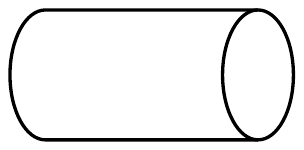
\includegraphics[width=2.4cm]{../gambar/simbol-4.png} & \textbf{\textit{Symbol Basisdata}} (simbol yang menunjukkan bahwa tempat penyimpanan data) \\
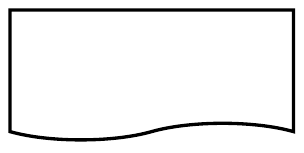
\includegraphics[width=2.4cm]{../gambar/simbol-5.png} & \textbf{\textit{Symbol Predefined Process}} (simbol untuk mempersiapkan penyimpanan yang akan digunakan sebagai tempat pengolahan di dalam \textit{storage}) \\
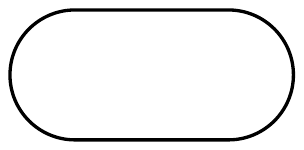
\includegraphics[width=2.4cm]{../gambar/simbol-6.png} & \textbf{\textit{Symbol Terminal}} (simbol untuk permulaan atau akhir dari suatu program) \\
\end{longtable}
\end{tanpagaris}

\subsection{Kesimpulan dan Saran}
\subsubsection{Kesimpulan}
Kesimpulan merupakan uraian singkat hasil penelitian dan pembahasan yang diperoleh (bukan kalimat statistik) dengan mengacu pada tujuan dan hipotesis penelitian yang dikaji.

\subsubsection{Saran}
Saran merupakan uraian atau anjuran yang mengacu pada kesimpulan penelitian yang dapat dimanfaatkan oleh pihak yang berkepentingan.

\section{Bagian Akhir}

\subsection{Daftar Pustaka}
Daftar pustaka memuat sumber informasi ilmiah yang diacu untuk menyusun laporan rencana penelitian, yang meliputi nama pengarang, tahun terbitan, judul, penerbit dan tempat penerbitan untuk buku. Untuk jurnal dicantumkan nama pengarang, tahun terbitan, judul artikel, nama dan nomor jurnal dan halaman. Sedangkan untuk pustaka yang diambil dari internet perlu dicantumkan nama pengarang, tahun terbit, judul artikel, alamat \textit{website} dan halaman diketik miring serta tanggal diakses. Daftar pustaka disusun berdasarkan urutan abjad nama pengarang.

Daftar pustaka berisi semua bahan pustaka yang dipakai penulis dalam penulisan skripsi. Kata DAFTAR PUSTAKA diketik dengan huruf kapital di bagian tengah halaman. Empat spasi di bawah kata DAFTAR PUSTAKA ditulis pustaka pertama. Tiap pustaka dimulai dari pinggir diketik satu spasi, baris kedua dan seterusnya dimulai pada ketukan ke delapan (\textit{tab stop} 0,5”). Jarak antara pustaka satu dengan lainnya dua spasi.

Pemakaian pustaka yang nama pengarangnya sama harus diketik dengan cara memberi garis yang panjangnya sama dengan nama pengarang di atasnya. Pustaka disusun menurut abjad dan tahun penerbitan. Apabila ada persamaan abjad maka didahulukan tahun yang lebih lama. Apabila nama sama dan tahun sama diberi tanda subskrip abjad di belakang tahun penerbitan. Pada daftar pustaka yang bersumber dari jurnal, penulisan judul hanya huruf pertama menggunakan huruf kapital, selanjutnya huruf kecil, kecuali kata-kata yang harus diketik dengan huruf kapital pada awal kata dan tidak dicetak miring walaupun dalam bahasa Inggris.

Penulisan pustaka yang berupa judul bab dari buku yang merupakan kumpulan banyak penulis ditulis dengan judul pertama huruf besar pada awal kalimat, selanjutnya huruf kecil, kecuali kata-kata yang harus diketik dengan huruf kapital pada awal kata, kemudian dilanjutkan dengan kata \textit{di dalam} atau \textit{In} dengan judul tiap kata diawali huruf besar.

\subsection{Lampiran}
LAMPIRAN disajikan setelah daftar pustaka; kata LAMPIRAN dimuat di bagian atas tengah halaman, ditulis dengan huruf besar. Isi lampiran adalah hasil penelitian skripsi yang tidak dimasukkan ke dalam tubuh tulisan agar tidak mengganggu uraian, umumnya berupa tabel yang melebihi satu halaman, peta lokasi penelitian, perhitungan statistik dan prosedur pendukung penelitian. Tiap topik lampiran diberi nomor urut dengan judul yang jelas. Judul lampiran ditulis dengan huruf kecil, kecuali awal kalimat huruf kapital dan tanpa titik di akhir kalimat.

% ============================ BAB III ============================
\chapter{FORMAT PENULISAN}

\section{Kertas}
Kertas yang dipergunakan adalah HVS ukuran A4 dengan berat kertas 80 g. Naskah asli sebagai pegangan mahasiswa yang bersangkutan, sedangkan untuk Fakultas, Jurusan/Program Studi dan keperluan lainnya dapat difotokopi dan diperbanyak dengan syarat fotokopi naskah bersih dengan halaman persetujuan bertanda tangan asli.

\section{Ketikan}
Naskah karya ilmiah diketik menggunakan komputer dengan program pengolah kata \textit{MS. Word} dengan huruf berjenis \textit{Times New Roman} berukuran 12 pt. Batas pengetikan 4 cm dari sisi kiri kertas, 4 cm dari sisi atas, 3 cm dari sisi kanan dan 3 cm dari bawah kertas, tidak termasuk nomor halaman. Pengaturan ketikan naskah dengan rata kanan-kiri (\textit{justify}).

Setiap alinea dimulai dengan \textit{tab stop} 0,5” (1,27 cm). Teks judul tabel, gambar dan daftar pustaka yang melebihi satu baris diketik satu spasi di bawah baris pertama. Setelah tanda titik dan koma diberi jarak satu ketukan. Jarak antara baris dalam teks adalah 2 spasi, sedangkan judul tabel, gambar dan lampiran jaraknya 1 spasi. Jarak ketikan naskah dengan anak bab berikutnya adalah 3 spasi. Setelah tanda koma dan titik dua diberi jarak 1 spasi (sebelum titik dua tidak diberi spasi), kecuali setelah tanda titik untuk kalimat baru, diberi jarak 1 spasi. Setiap bab dimulai pada halaman baru, diketik dengan huruf kapital dan diletakkan di tengah atas halaman. Subbab diketik di pinggir sisi kiri halaman, dengan huruf kecil kecuali huruf pertama pada setiap kata diketik dengan huruf kapital. Pemutusan kata dalam satu baris kalimat harus mengikuti kaidah bahasa Indonesia yang baku dan benar.

\section{Cetak Miring}
Kata-kata bahasa di luar bahasa Indonesia baku ditulis miring, misalnya bahasa Inggris, Latin dan lain-lain.

\section{Tabel}
Suatu tabel harus dimuat dalam satu halaman, tidak boleh diputus atau dilanjutkan pada halaman berikutnya. Nomor tabel disusun seperti nomor gambar, yaitu nomor bab dan nomor urut tabel di bab itu (Tabel 1.1, Tabel 3.2); pada lampiran memakai awalan nomor lampiran (Tabel L2.1). Judul tabel harus mudah dimengerti dan ditulis dengan jarak 1 spasi dan huruf kapital hanya pada awal kalimat dan diakhiri tanpa titik. Sumber data yang termuat dalam tabel harus disebutkan dan ditulis sesudah garis bawah tabel dengan jarak 1 spasi.

\section{Gambar}
Gambar meliputi: grafik, diagram, monogram, foto, peta, skema. Nomor gambar terdiri atas nomor bab dan nomor urut gambar di bab itu, dipisahkan titik. Contoh: Gambar 1.1. Data populasi adalah gambar pertama pada Bab I, dan Gambar 2.3 adalah gambar ketiga pada Bab II. Gambar pada lampiran diberi awalan nomor lampiran, misalnya Gambar L2.1. Huruf selain huruf pertama dari kata pertama dalam kalimat menggunakan huruf kecil dan judul gambar diletakkan di bawah gambar. Judul keterangan gambar dibuat dengan jarak 1 spasi.

\section{Penyusunan dan Penomoran Halaman}
Susunan lembaran skripsi dimulai dari halaman sampul sampai lampiran, berturut-turut diatur sebagai berikut:
\begin{enumerate}
\item Halaman sampul depan
\item Halaman pengajuan
\item Halaman pengesahan
\item Halaman kata pengantar
\item Halaman daftar isi
\item Halaman daftar tabel
\item Halaman daftar gambar
\item Halaman daftar lampiran
\item BAB I Pendahuluan
\item BAB II Tinjauan Pustaka
\item BAB III Metode Penelitian
\item BAB IV Hasil dan Pembahasan
\item BAB V Kesimpulan dan Saran
\item Daftar Pustaka
\item Halaman Lampiran
\end{enumerate}

\section{Angka dan Satuan}
Angka dan satuan pada awal kalimat harus ditulis dengan kata, tetapi angka yang diikuti bulan, nomor halaman, persen, waktu, dan satuan tetap ditulis dengan angka, misalnya: 1 Januari 1988; 37°C; halaman 37; 5\%; 10.30 WIB (tanda titik khusus untuk waktu) dan 8 cm. Angka bilangan bulat sampai dengan sepuluh harus ditulis dengan kata kecuali diikuti dengan satuan (kg, cm), tetapi jika lebih dari sepuluh ditulis biasa, misalnya: delapan; 2 cm; 15; 20 cm dst.

Angka yang menyatakan desimal menggunakan tanda koma (1,50 kg). Ribuan atau kelipatan ribuan ditulis dengan tanda titik setiap tiga angka, misalnya: 1.000 m; 100.000 ekor. Dalam satu tabel, jumlah digit di belakang koma harus konsisten (dengan melihat jenis variabel yang diukur) apabila dicantumkan dalam satu tabel.

\section{Pemisahan Kata di Akhir Baris}
Pemenggalan kata pada akhir baris harus disesuaikan dengan tata bahasa yang benar. Batas sebelah kiri dan sebelah kanan harus lurus, kata di dalam kalimat dapat direnggangkan paling banyak tiga ketukan. Kata sambung di akhir halaman diikutkan pada halaman berikutnya.

\section{Alinea}
Alinea merupakan bagian dari bab atau subbab yang menceritakan suatu pernyataan tertentu dan berisi satu ide. Penulisan alinea dimulai ketukan keenam (\textit{tab stop} 0,5”) dari batas kiri. Jika alinea yang tertulis di baris akhir di suatu halaman hanya berisi satu baris, hal itu tidak dibenarkan, oleh karena itu perlu dipindah ke halaman berikutnya. Pada akhir halaman minimal tercantum dua baris.

\section{Tabel dan Gambar}
Tabel, gambar, grafik, foto harus dimuat pada halaman yang sama dan tidak boleh diputus. Tabel yang panjang (lebih dari satu halaman) diletakkan di dalam lampiran. Tabel merupakan hasil penelitian yang sudah diolah/dianalisis, sedangkan gambar di dalam ilustrasi berupa foto, grafik, struktur organisasi, alur kerja dan proses. Kata tabel dan gambar yang diikuti nomor urut dalam naskah selalu diawali dengan huruf kapital. Nomor urut tidak boleh ditulis dengan kata. Kata tabel, nomor, dan judul dimulai tiga spasi di bawah teks pada halaman yang bersangkutan. Tabel dibuat satu spasi di bawah judul tabel. Garis yang dipakai untuk membuat tabel adalah garis tunggal yang membentuk kotak penuh (garis atas, bawah, kiri, kanan, dan antarbaris). Isi tabel diketik satu spasi. Tabel yang berasal dari data sekunder disebutkan sumbernya, yang ditulis satu spasi di bawah garis bawah tabel yang bersangkutan. Gambar di dalam penulisan skripsi sama peraturannya seperti pembuatan tabel, tetapi judulnya diletakkan dua spasi di bawah gambar.

\section{Kutipan}
Kutipan yang ditulis pada skripsi harus sesuai dengan maksud dari tulisan pada pustaka yang diambil. Penempatan nama pengarang bisa di depan, tengah atau akhir kalimat. Nama orang yang ditulis:
\begin{enumerate}[a.]
\item Di depan kalimat: Sastra (1994) menyatakan bahwa …; Jones (1993) melaporkan bahwa … atau Menurut Adams (2000), daging juga mengandung … dst.
\item Di bagian tengah kalimat: … diketahui oleh Jones (1982), Arey (1993) dan Edey \textit{et al.} (1988) bahwa: … dst.
\item Di akhir kalimat: … kotoran ternak masih mempunyai nilai nutrisi sebagai pakan ternak … (Fontenot \textit{et al.}, 1993).
\end{enumerate}
Singkatan \textit{et alii} adalah \textit{et al.}, dipakai apabila pengarangnya bukan orang Indonesia. Singkatan \textit{dan kawan-kawan} adalah \textit{dkk.}, dipakai apabila pengarangnya orang Indonesia. Pada pengutipan pertama, nama penulis harus dicantumkan secara lengkap. Penggunaan singkatan tersebut berlaku apabila penulisnya lebih dari dua orang dan ditulis setelah kutipan kedua kali dan seterusnya. Penulisan pustaka tanpa pengarang ditulis Anonimous; apabila nama pengarang tidak ada tetapi ada lembaga yang mengeluarkan, maka ditulis nama lembaganya.

% ============================ BAB IV ============================
\chapter{PENUTUP}

Skripsi yang telah disetujui oleh pembimbing dapat dilanjutkan dengan ujian. Apabila mahasiswa dinyatakan lulus dan telah melakukan revisi dengan persetujuan penguji dan pembimbing, maka dapat dilanjutkan dengan penjilidan skripsi. Penjilidan dengan menggunakan jilid skripsi standar berwarna biru laut yang dilaminasi. Skripsi disahkan oleh Pembimbing I, Pembimbing II, Ketua Program Studi dan Dekan Fakultas Teknik Universitas Muhammadiyah Buton.

% ============================ LAMPIRAN ============================
\lampiran{1}{Contoh kata pengantar}
\begin{tengah}
\textbf{KATA PENGANTAR}
\end{tengah}

Puji syukur penulis panjatkan kepada Allah Yang Maha Kuasa, sehingga dapat menyelesaikan penulisan skripsi ini. Untuk itu penulis juga sangat berterima kasih kepada yang terhormat:
\begin{enumerate}
\item Nama Pembimbing 1, selaku Pembimbing Utama dan Nama Pembimbing 2, selaku Pembimbing Pendamping atas saran dan bimbingannya.
\item Nama Dekan Fakultas Teknik, selaku Dekan Fakultas Teknik Universitas Muhammadiyah Buton.
\item Nama Ketua Program Studi, selaku Ketua Program Studi yang telah banyak membina kelancaran proses studi.
\item Nama Penguji 1 dan Nama Penguji 2, selaku penguji atas masukan dan saran selama Ujian Sarjana.
\item Penulis juga menyampaikan terima kasih kepada ………… (pihak terkait yang mendukung penyelesaian skripsi).
\end{enumerate}

\begin{kanan}
Baubau, November 2015

(Penulis)
\end{kanan}

\lampiran{2}{Contoh penulisan gambar dan tabel}
\textit{LVDT} ditempatkan pada puncak kolom, tengah kolom dan bawah kolom yang dimaksudkan sebagai data pengontrol nantinya dalam pengolahan hasil pengujian. Dua buah \textit{LVDT} juga ditempatkan pada balok untuk melihat \textit{displacement} yang terjadi pada daerah \textit{grouting}.

\begin{figure}[H]
\centering
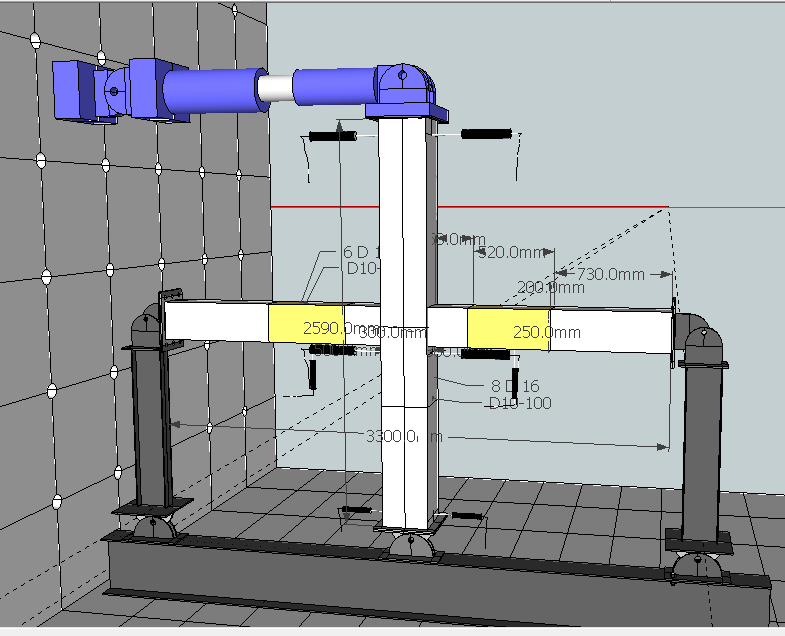
\includegraphics[width=0.5\textwidth]{../gambar/contoh-lvdt.png}
\caption{Detail penempatan \textit{LVDT}}
\end{figure}

\needspace{9cm}
Tabel L2.1 di bawah ini menyajikan resume data benda uji, termasuk di dalamnya ukuran penampang balok-kolom dan properti material penyusun yang nantinya merupakan dasar dalam pengolahan hasil pengujian.

\begin{singlespace}
\setlength{\tabcolsep}{10pt}
\begin{longtable}{|p{0.34\linewidth}|c|c|c|}
\caption{Resume data benda uji}\\
\hline
\textbf{Deskripsi} & \textbf{Balok} & \textbf{Kolom} & \textbf{\textit{Grouting}} \\
\hline
Panjang (L) & 3300 mm & 2950 mm & 520 mm \\
\hline
Tinggi (h) & 250 mm & 300 mm & 250 mm \\
\hline
Lebar (b) & 200 mm & 300 mm & 200 mm \\
\hline
Selimut (d) & 40 mm & 40 mm & 40 mm \\
\hline
f’c & 25 MPa & 25 MPa & 50 MPa \\
\hline
Diameter tulangan utama & 13 mm & 16 mm & 13 mm \\
\hline
Fy tulangan utama & 300 MPa & 300 MPa & 300 MPa \\
\hline
Diameter sengkang & 10 mm & 10 mm & 10 mm \\
\hline
Fy tulangan sengkang & 400 MPa & 400 MPa & 400 MPa \\
\hline

\end{longtable}
\end{singlespace}

\lampiran{3}{Contoh daftar tabel}
\begin{tengah}
\textbf{DAFTAR TABEL}
\end{tengah}
\begin{tanpagaris}
\begin{longtable}{@{}p{0.13\linewidth}p{0.67\linewidth}r@{}}
\textbf{Nomor} & \textbf{Judul} & \textbf{Halaman} \\
1 & Resume data benda uji & 2 \\
\end{longtable}
\end{tanpagaris}

\lampiran{4}{Contoh daftar gambar}
\begin{tengah}
\textbf{DAFTAR GAMBAR}
\end{tengah}
\begin{tanpagaris}
\begin{longtable}{@{}p{0.13\linewidth}p{0.67\linewidth}r@{}}
\textbf{Nomor} & \textbf{Judul} & \textbf{Halaman} \\
1 & Beberapa pola kurva histeresis & 5 \\
2 & Mekanisme plastifikasi rangka & 9 \\
\end{longtable}
\end{tanpagaris}

\lampiran{5}{Contoh daftar lampiran}
\begin{tengah}
\textbf{DAFTAR LAMPIRAN}
\end{tengah}
\begin{tanpagaris}
\begin{longtable}{@{}p{0.13\linewidth}p{0.67\linewidth}r@{}}
\textbf{Nomor} & \textbf{Judul} & \textbf{Halaman} \\
1 & Proses perakitan besi & 63 \\
2 & Proses pembuatan bekisting & 63 \\
3 & Pemasangan \textit{strain gauge} setelah pengelasan & 64 \\
4 & Persiapan pengecoran & 65 \\
5 & Proses pengecoran & 65 \\
6 & Pekerjaan persiapan tiang \textit{support} & 66 \\
7 & Tulangan yang akan di-\textit{grouting} & 66 \\
8 & Proses persiapan benda uji untuk melakukan \textit{grouting} pada sambungan & 67 \\
9 & Detail tulangan pada daerah \textit{grouting} & 67 \\
10 & Permukaan beton yang akan di-\textit{grouting}, dibersihkan kemudian dilapisi dengan \textit{epoxy} & 68 \\
11 & Proses \textit{grouting} & 68 \\
12 & Proses pengujian benda uji konvensional & 69 \\
13 & Proses pengujian benda uji \textit{grouting} & 69 \\
14 & Proses pengujian benda uji konvensional & 70 \\
15 & Kerusakan pada benda uji \textit{grouting} & 70 \\
\end{longtable}
\end{tanpagaris}

\lampiran{6}{Contoh daftar pustaka}
\begin{tengah}
\textbf{DAFTAR PUSTAKA}
\end{tengah}
\begin{pustaka}
Anonimus. 2008. Komposisi kimia ekstrak kulit jeruk. \textit{http://www.jeruk.com}. Diakses tanggal: 22 Juli 2008.

—————— 2008. Komposisi kimia ekstrak jahe. \textit{http://www.jeruk.com}. Diakses tanggal 22 Juli 2008.

Bennet, C. 1999. Cooperative Extention Roles and Relationships for New Era: Extention Service. US Department of Agriculture. Washington DC.

BPS, 1997. Statistik Indonesia 1996. Badan Pusat Statistik. Jakarta.

Gardjito, M., S. Nambi, Murdiati dan Sujono, 1994. Ilmu Pangan. Terjemahan dari The Science of Food oleh Gaman P.M. and K.B. Sherrington. Gadjah Mada University Press. Yogyakarta.

Idris, M. 1994. Pembuatan telur asin dengan cara penyuntikan. Poultry Indonesia 176: 18-19.

Kailasepathy, K. 1996. Polysaccharide ingredients in dairy products application: increase in cheese yield. J. Food Australia 48 (10): 58-461.

Lim, J.M., J.J. Hwang, H.M. Chung and K. Niwa. 1999. Development of \textit{in vivo} maturated bovine oocytes rafter cryopreservative with different cryoprotectants. J. Theriogernology 51: 1303-1310.

NRC. 1989. Nutrient Requirements of Dairy Cattle. National Research Council. 6th Revised Edition. NRC. Washington.

Radiati, L.E. 2000. Penghambatan bakteri enteropatogen oleh ekstrak jahe. J. Habitat. 12 (2): 81-91.
\end{pustaka}

\end{document}
